%--------------------
% Packages
% -------------------
\documentclass[12pt,a4paper]{article}
% \usepackage[a4paper, left=15mm, right=15mm, top=15mm, bottom=15mm]{geometry}
\usepackage[utf8x]{inputenc}
\usepackage[T1]{fontenc}
%\usepackage{gentium}
\usepackage{mathptmx} % Use Times Font
% \usepackage[siunitx]{circuitikz} % for circuit schematics
\usepackage{siunitx}
\usepackage{amsmath} % for the equation* environment


\usepackage[pdftex]{graphicx} % Required for including pictures % clashes with circuitikz
% \usepackage[swedish]{babel} % Swedish translations
\usepackage[pdftex,linkcolor=black,pdfborder={0 0 0}]{hyperref} % Format links for pdf
\usepackage{calc} % To reset the counter in the document after title page
\usepackage{enumitem} % Includes lists

\frenchspacing % No double spacing between sentences
\linespread{1.2} % Set linespace
\usepackage[a4paper, lmargin=0.08\paperwidth, rmargin=0.08\paperwidth, tmargin=0.08\paperheight, bmargin=0.08\paperheight]{geometry} %margins
%\usepackage{parskip}
% \usepackage[all]{nowidow} % Tries to remove widows
\usepackage[protrusion=true,expansion=true]{microtype} % Improves typography, load after fontpackage is selected

\usepackage[inkscapelatex=false]{svg}
\graphicspath{ {./media/} }

% \pagecolor{black}
% \color{white}

\usepackage{setspace}


%-----------------------
% Set pdf information and add title, fill in the fields
%-----------------------
\hypersetup{ 	
pdfsubject = {},
pdftitle = {ee5311-2025-ee24s053-pwc-report-tut2},
pdfauthor = {Karthik B K <ee24s053@smail.iitm.ac.in>}
}

%-----------------------
% Begin document
%-----------------------
\begin{document}

\title{EE5311 \\ Report of Practical Work Conducted for Tutorial 02}
\author{Karthik B K ee24s053}
\maketitle

\section{Experiment 01}
\subsection{Calculations}
In the given circuit schematic, we know from visual inspection that the pMOS's region of operation will be \emph{saturation} and that of the nMOS will be \emph{linear}. With that information, we equate the currents in the said regions of operations as follows:

\doublespacing
\begin{center}
    $I_{d,sat,p} = I_{d,lin,n}$
\end{center}
\begin{center}
    $\frac{1}{2}\mu_{p}C_{ox}(\frac{W}{L})_{p}\frac{E_{C}L(V_{gs}-V_{tp})^{2}}{V_{gs}-V_{tp}+E_{C}L}(1+\lambda_{p} V_{ds}) = $\\$\frac{1}{2}\mu_{n}C_{ox}(\frac{W}{L})_{n}\frac{1}{1+(\frac{V_{ds}}{E_{C}L})}(2(V_{gs}-V_{tn})V_{ds}-V_{ds}^2)(1+\lambda_{n} V_{ds})$
\end{center}
\singlespacing

\noindent We use the values provided in the problem statement, and obtain:

\doublespacing
\begin{center}
    $(\frac{W}{L})_{p} = 1.610$
\end{center}
\singlespacing

\noindent Since the minimum width of a 3-terminal pMOS transistor in the given sky130 standard cell library is $0.42 \mu m$, we want to increase the length of our pMOS device to meet this aspect ratio. Hence, we would size the pMOS transistor as follows:

\doublespacing
\begin{center}
    $W_{p} = 0.42 \mu m, L_{p} = 0.26 \mu m$
\end{center}
\singlespacing

\noindent In order to compute the noise margins, we first compute $V_{IH}$ and $V_{IL}$ as follows:

\doublespacing
\begin{center}
    $V_{IL} = V_{tn} + \frac{1}{R_L(2k_n\frac{W_n}{L_n})}$ \\
    $V_{IH} = V_{tn} + \sqrt{\frac{4V_{DD}}{3K_nR_L\frac{W_n}{L_n}}} - \frac{1}{2K_nR_L\frac{W_n}{L_n}}$
\end{center}
\singlespacing

\noindent We use the values provided in the problem statement, and obtain:

% \doublespacing
\begin{center}
    $V_{IL} = 0.765 mV$ \\
    $V_{IH} = 1196 mV$
\end{center}
% \singlespacing

\begin{equation}
    \label{eq:expt1-noise-margins}
    NM_L = 0.765V, NM_H = 0.604V
\end{equation}

\noindent In order to compute average power at a constant onput voltage level, $V+{in} = V_{DD}$, we can simply measure the current drawn from the voltage source $V_{DD}$ and multiply it with the maginitude of the supply voltage level, $1.8V$.
Since the gate terminal of the pMOS device is fixed to the ground voltage level, the pMOS device remains in saturation and thus there is a constant current being drawn from the supply, which is of the magnitude:

\doublespacing
\begin{center}
    $I_{d,sat,p} = \frac{1}{2}\mu_{p}C_{ox}(\frac{W}{L})_{p}\frac{E_{C}L(V_{gs}-V_{tp})^{2}}{V_{gs}-V_{tp}+E_{C}L}(1+\lambda_{p} V_{ds})$ %and \\
    %$I_{d,lin,n} = \frac{1}{2}\mu_{n}C_{ox}(\frac{W}{L})_{n}\frac{1}{1+(\frac{V_{ds}}{E_{C}})}(2(V_{gs}-V_{tn})V_{ds}-V_{ds}^2)(1+\lambda_{n} V_{ds})$
\end{center}
\singlespacing

\noindent We use the values provided in the problem statement, and approximate $E_CL$ to be equal to $1$. We obtain,

\doublespacing
\begin{center}
    $I_{d,sat,p} = 49.61 \mu A$ %and \\
    %$I_{d,lin,n} = 291.9 \mu A$ \\
    %$thus, $I_{out} = -291.1 \mu A$ \\
    %$indicating $P_* = abs(I_{out}) * V_{DD} = 678.8 \mu W$
\end{center}
\singlespacing

\noindent Once the input voltage becomes larger than the nMOS threshold voltage level, the nMOS starts conducting current, essentially reducing the amount of current going to the output pin. However, pMOS continues to conduct the same amount of current. Thus, the power consumed can be approximated as:

% \doublespacing
\begin{center}
    $P_* = I_{d,sat,p} * V_{DD}$
    % $P_* \approx 154.98 \mu W$
\end{center}
% \singlespacing

\begin{equation}
    \label{eq:expt1-avg-power}
    P_{avg} = 89.298 \mu W
\end{equation}

\subsection{Schematics}
\noindent We draw the following schematic using \emph{xschem}.
\newline
\begin{center}
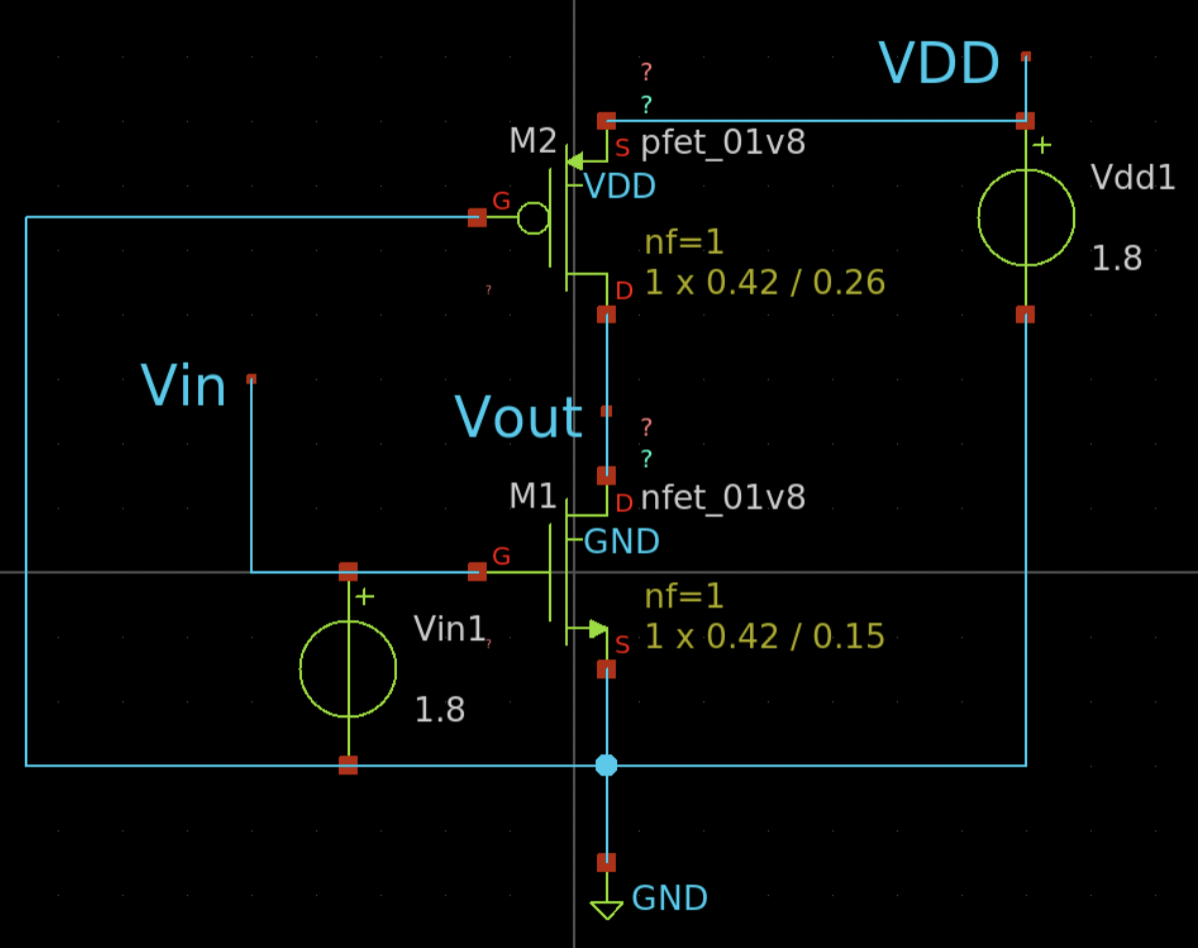
\includegraphics[scale=0.4]{tut2/reports/media/expt1.sch.png} \\ Fig 1: Schematic of the pseudo-inverter.
\end{center}


\subsection{Measurements}

\noindent We plot the voltage transfer charecteristics for the said inverter using a SPICE simulation and obtain the following plot:

\begin{center}
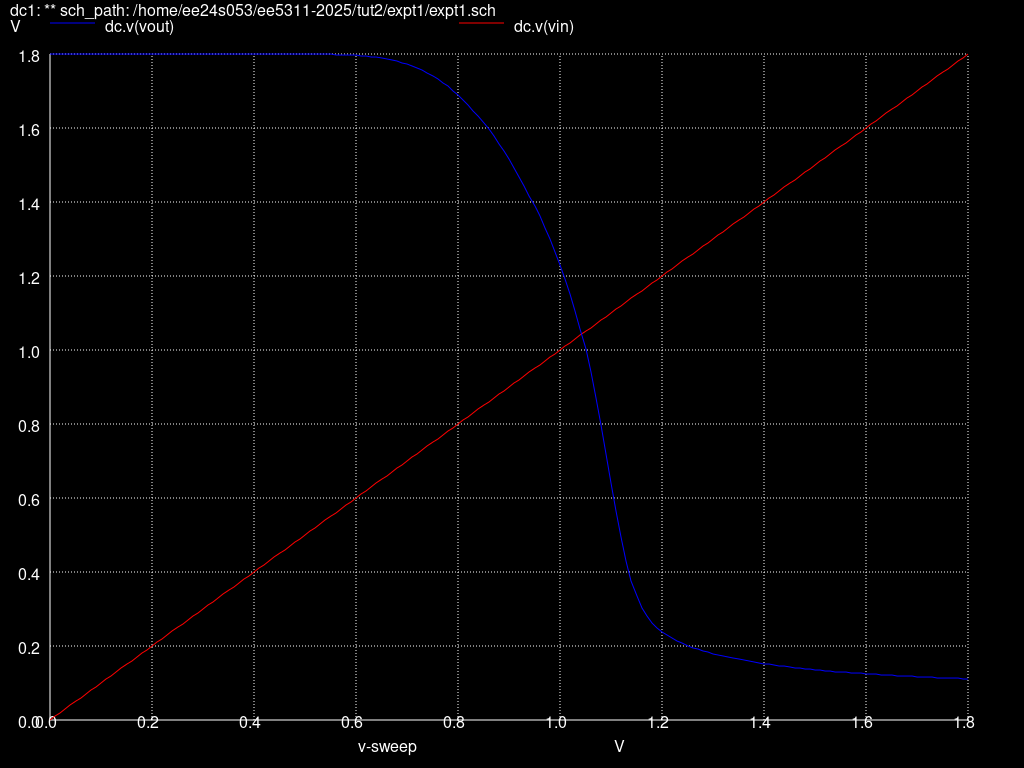
\includegraphics[scale=0.3]{tut2/reports/media/expt1_vtc.png} \\ Fig 2: Voltage Transfer Charecteristics of the pseudo-inverter.
\end{center}

\noindent We measure the inverter threshold voltage, defined as the magnitude of input voltage for which the output voltage is half of the supply voltage, as follows:

\begin{verbatim}
    meas dc Vtinv when v(Vout)=0.9 cross=1
\end{verbatim}

\noindent We observe that the inverter voltage is: $1.06587$ V.\newline
We also plot the first-order derivative of the output voltage curve using a SPICE simulation and obtain the following plot:

\begin{center}
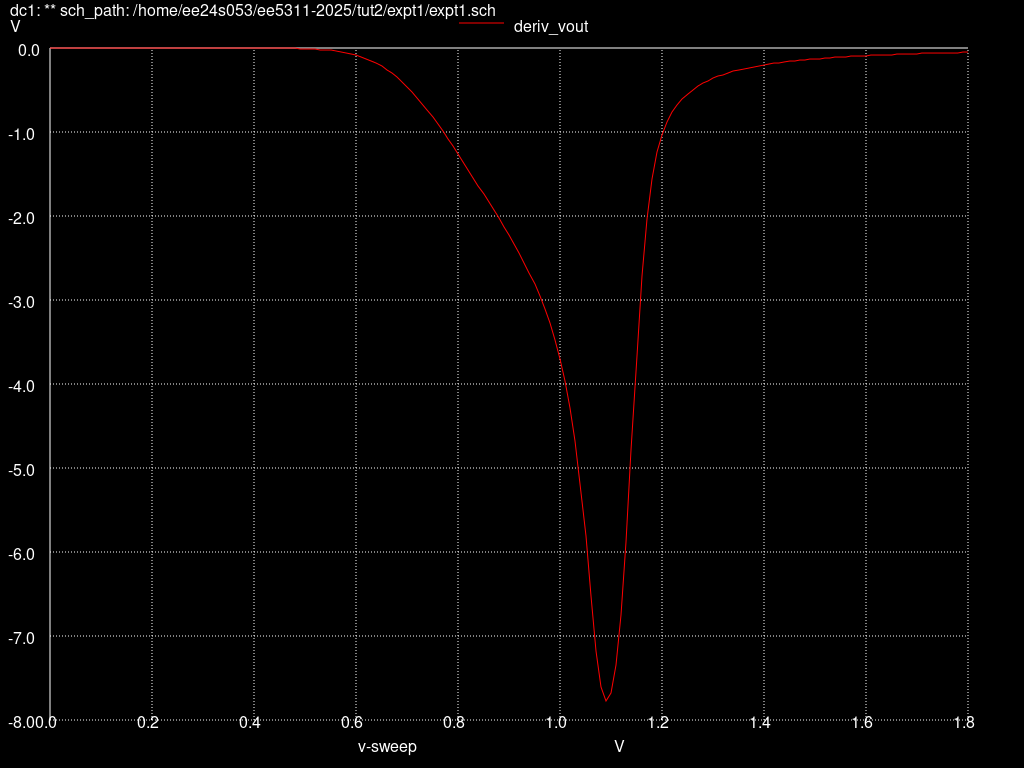
\includegraphics[scale=0.3]{tut2/reports/media/expt1_deriv_vout.png} \\ Fig 3: First-Order Derivative of the Output Voltage across a range of input voltages.
\end{center}

\noindent We measure the input voltage levels, $Vil, Vih$, as follows:

\begin{verbatim}
    let deriv_vout = deriv(v(Vout))
    meas dc Vil when deriv_vout=-1 cross=1
    meas dc Vih when deriv_vout=-1 cross=2
\end{verbatim}

\noindent We obtain the following values:

\begin{verbatim}
    vil = 7.707750e-01
    vih = 1.202181e+00
\end{verbatim}

\noindent Using these values for $Vil, Vih$, we compute the noise margins, $NM_{L}$ and $NM_{H}$ to be:

\begin{verbatim}
    NML: 0.770775
    NMH: 0.597819
\end{verbatim}

\noindent We compare these values with (\ref{eq:expt1-noise-margins}) and notice a variation of upto 0.01 V.
\newline
\noindent Given that $V_{in} = V_{dd}$, we can say that the average power consumed will be equal to the peak power consumed, which is $P_* = I_{out} * V_{dd}$. In order to compute this, we \emph{simply} fix the input voltage level to what is asked, $V_{dd}$ and measure the current drawn from the supply voltage. We plot the output current throughout the DC sweep, and measure the value of current at the said input voltage level. We obtain the following plot:

\begin{center}
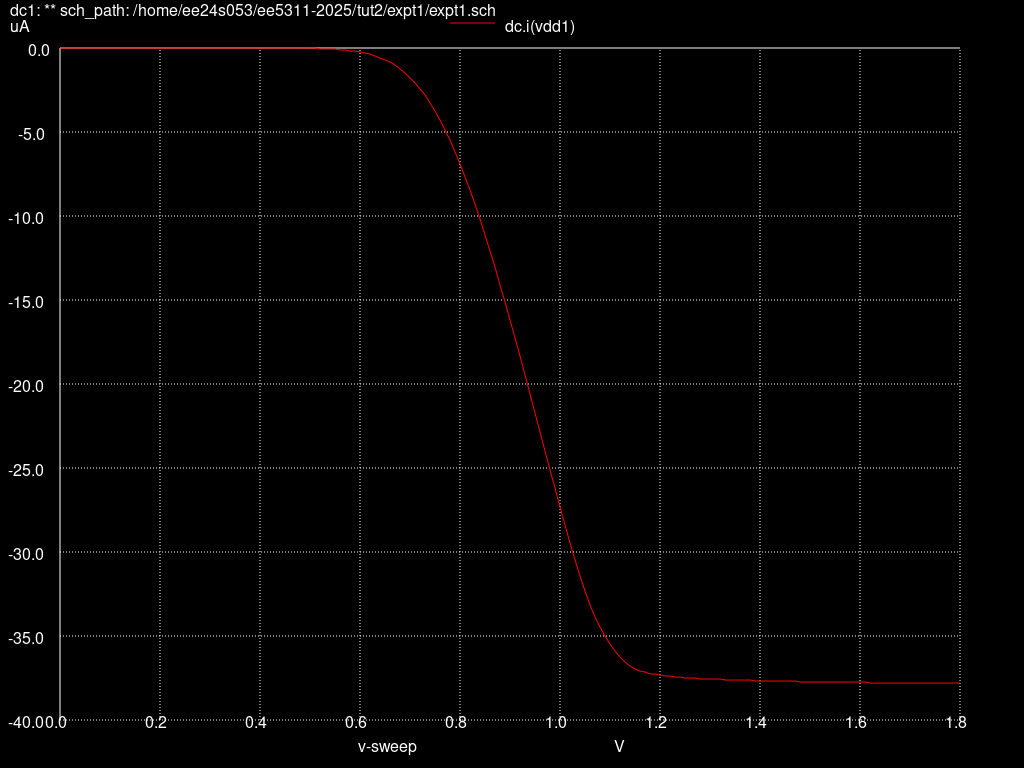
\includegraphics[scale=0.3]{tut2/reports/media/expt1_iout.png} \\ Fig 4: Output Current for a range of input voltages.
\end{center}

\noindent At $V_{in} = V_{dd}$, we obtain the following measurement for the current:

\begin{verbatim}
    Iout = 3.781284e-05
\end{verbatim}

\noindent Hence,
\doublespacing
\begin{center}
    $P_* = 3.781 * 10^{-5} * 1.8 W = 6.805 * 10^{-5} W$
\end{center}
\doublespacing
\noindent The average power consumed when $V_{in} = V_{dd}$ is:
\doublespacing
\begin{center}
    $P_* = 68.05 \mu W$
\end{center}
\singlespacing
\noindent We compare this value with (\ref{eq:expt1-avg-power}) and notice some difference in the power consumption.

\section{Experiment 02}
\subsection{Calculations}
\noindent When the inverter threshold voltage level is desired to be half that of the supply voltage, $V_{tinv} = V_{m} = \frac{V_{DD}}{2}$, both the transistors are going to be in saturation, since $V_{DS} = V_{GS} \rightarrow V_{DS} > V_{GS} - V_T$. We equate the drain currents, $I_{D_N} = I_{D_P} : V_M \approx \frac{rV_{DD}}{1+r}$ where $r = \frac{k_pV_{D,sat,p}}{k_nV_{D,sat,n}}$ such that $r=1$.

\doublespacing
\begin{center}
    $\frac{(W/L)_p}{(W/L)_n} = \frac{k_nV_{D,sat,n}(V_m-V_{T_n} - (V_{D,sat,n}/2))}{k_pV_{D,sat,p}(V_{DD}-V_m+V_{T_p} + (V_{D,sat,p}/2))}$
    %$I_{d,sat,p} = I_{d,lin,n}$ \\
    %$\frac{1}{2}\mu_{p}C_{ox}(\frac{W}{L})_{p}\frac{E_{C}(V_{gs}-V_{tp})^{2}}{V_{gs}-V_{tp}+E_{C}}(1+\lambda_{p} V_{ds}) = $\\$\frac{1}{2}\mu_{n}C_{ox}(\frac{W}{L})_{n}\frac{1}{1+(\frac{V_{ds}}{E_{C}})}(2(V_{gs}-V_{tn})V_{ds}-V_{ds}^2)(1+\lambda_{n} V_{ds})$
\end{center}
\singlespacing

\noindent We use the values provided in the problem statement, and obtain:

\doublespacing
\begin{center}
    $(\frac{W}{L})_{p} = 1.133$
\end{center}
\singlespacing

\noindent In order to retain symmetricity in sizing, we will size the pMOS to be the next multiple of the nMOS width. Hence, $W_p = 0.84 \mu m$ and $L_p = 0.15 \mu m$. The nMOS device remains to be a minimum-sized transistor.
\newline\newline
\noindent We simply compute the drain current, $I_D$ for the pMOS being in saturation in order to determine the maximum current. We use the following equation when $V_{DD} = 0.2 V$. We compute $I_S$ using the analytical model for pMOS current in saturation.

\doublespacing
\begin{center}
    $I_{D,subvt} = I_S \cdot e^{\frac{V_{gs}-V_T}{nV_T}} \cdot (1-e^{\frac{-V_{DS}}{V_T}})$ \\
    using $V_T \approx 26 mV$, $I_S = 10.207 \mu A$ and $n=1$, we get
\end{center}
\singlespacing

\begin{equation}
    \label{eq:expt2-idmax-subvt}
    I_{D,max,subvt} = -1.71 pA
\end{equation}

\noindent Similarly, we calculate the maximum draincurrent when the supply voltage, $V_{DD} = 0.8 V$.

\begin{equation}
    \label{eq:expt2-idmax-nearvt}
    I_{D,max,nearvt} = ?A
\end{equation}

\noindent Similarly for $V_{DD} = 1.8 V$.
\begin{equation}
    \label{eq:expt2-idmax-supervt}
    I_{D,max,supervt} = ?A
\end{equation}

\subsection{Schematics}
\noindent We draw the following schematic using \emph{xschem}:
\begin{center}
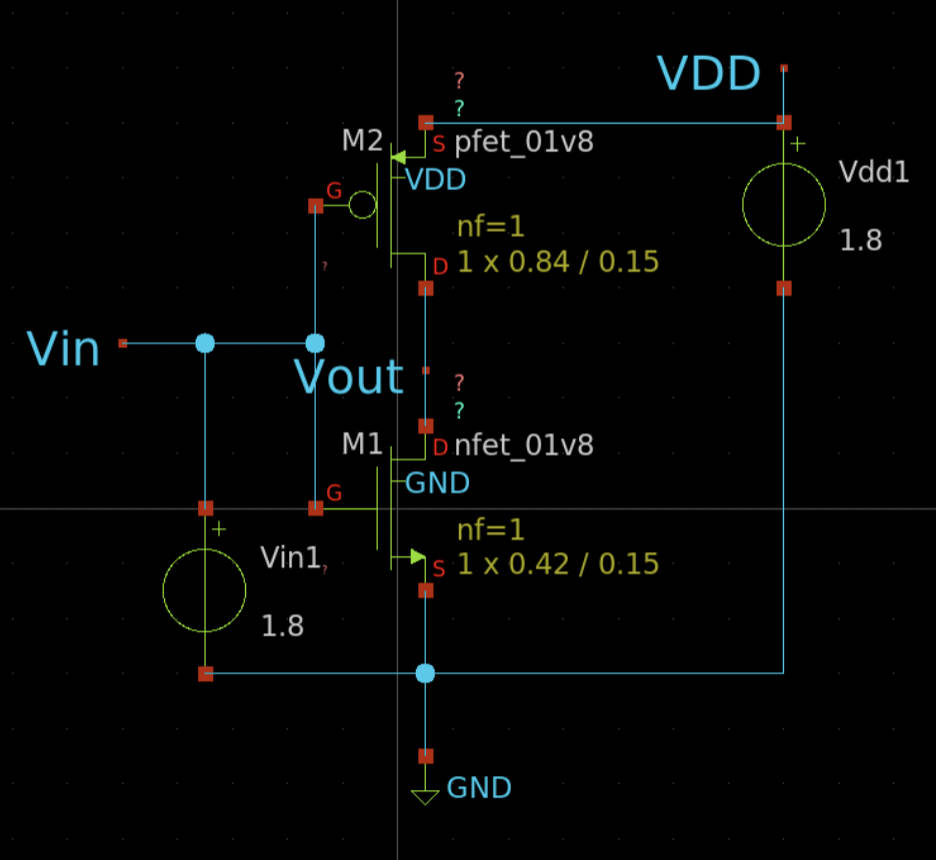
\includegraphics[scale=0.7]{tut2/reports/media/expt2_0.sch.png} \\ Fig 5: Schematic of the Symmetric CMOS Inverter.
\end{center}

\subsection{Measurements}
\noindent We obtain the following plot for voltage transfer characteristics:
\begin{center}
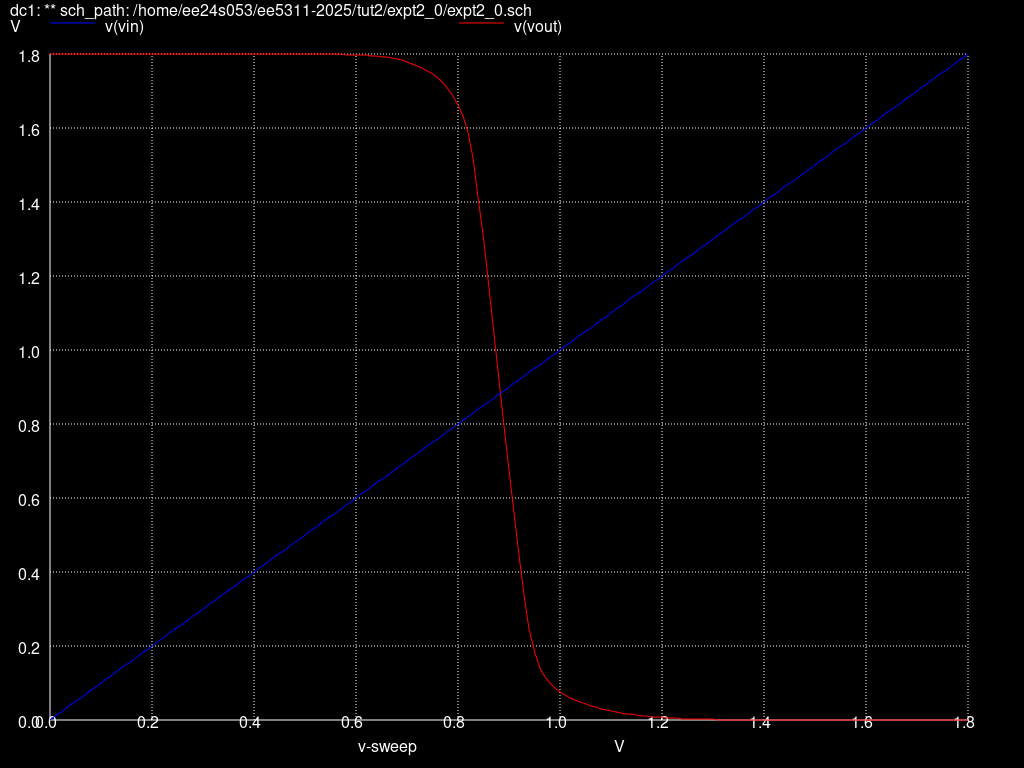
\includegraphics[scale=0.35]{tut2/reports/media/expt2_0_vtc.png} \\ Fig 6: Voltage Transfer Characteristics of the Symmetric CMOS Inverter.
\end{center}

\noindent By visual inspection, we note that the $V_M$ obtained through simulation is close to $0.9V$, close to our design target. We obtain the following plot for the derivative of the output voltage level:

\begin{center}
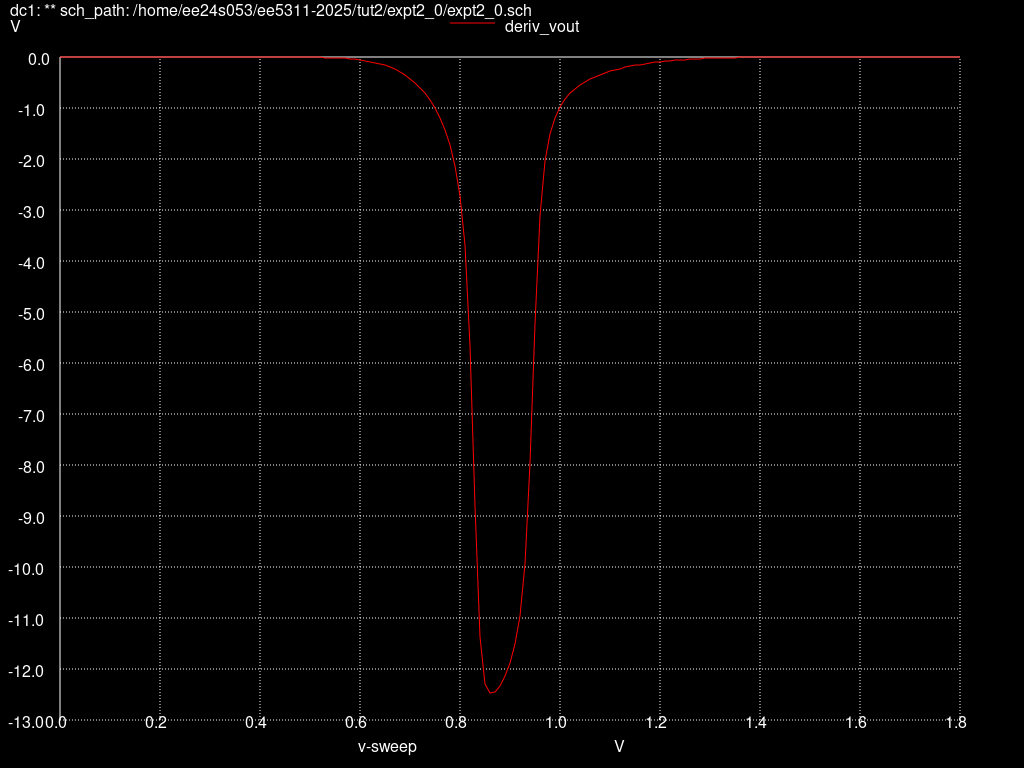
\includegraphics[scale=0.35]{tut2/reports/media/expt2_0_deriv_vout.png} \\ Fig 7: First-Order Derivative of the Output Voltage for a Symmetric CMOS Inverter.
\end{center}

\noindent If we increase the size of our pMOS transistor, then the VTC curve will shift to the right, since the nMOS will not be able to handle all that current from the pull-up circuit easily. If we down-size the pMOS, then the VTC curve will shift to the left.

\noindent We make the following measurements from the plotted curve:

\doublespacing
\begin{center}
    $V_{IL} = 750.0234 mV$ \\
    $V_{IH} = 999.1007 mV$ \\
    $V_m = 881.4951 mV$ \\
    thus, $NM_L = 750.023 mV$ and $NM_H = 800.899 mV$
\end{center}
\singlespacing

\noindent We modify the simulation setup to sweep the supply voltage level from $0.2V$ to $1.8V$ in steps of $0.2V$. We obtain the following voltage transfer characteristics:
\begin{center}
\begin{tabular}{cc}
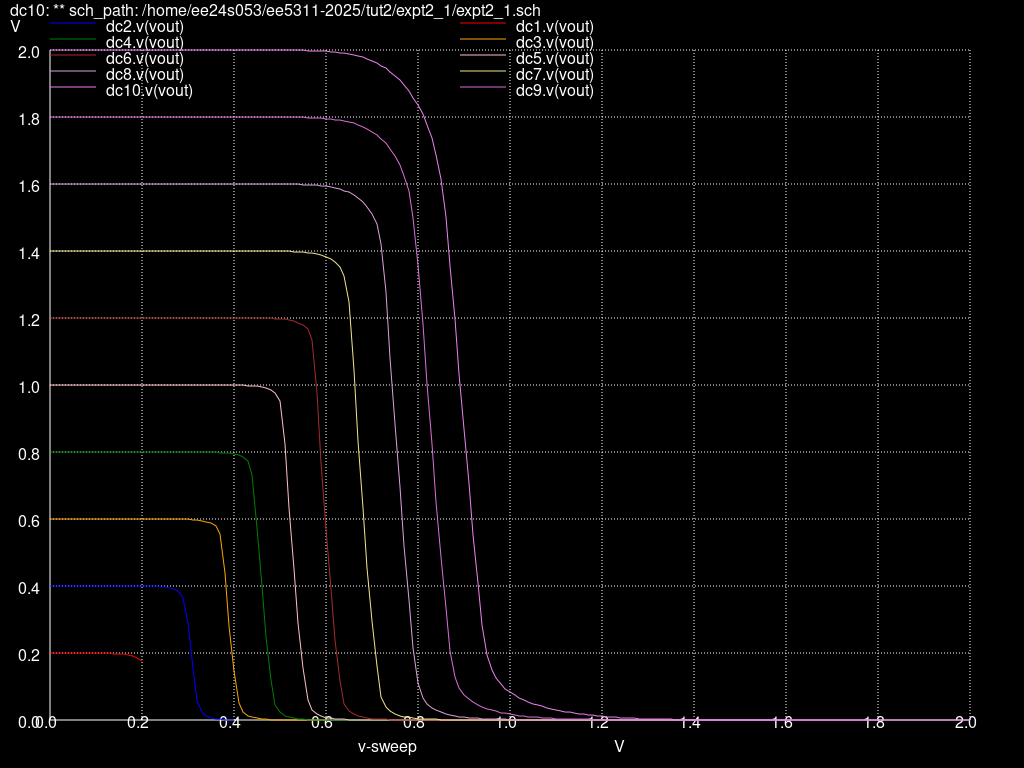
\includegraphics[width=0.49\linewidth]{tut2/reports/media/expt2_1_vtc.png} &
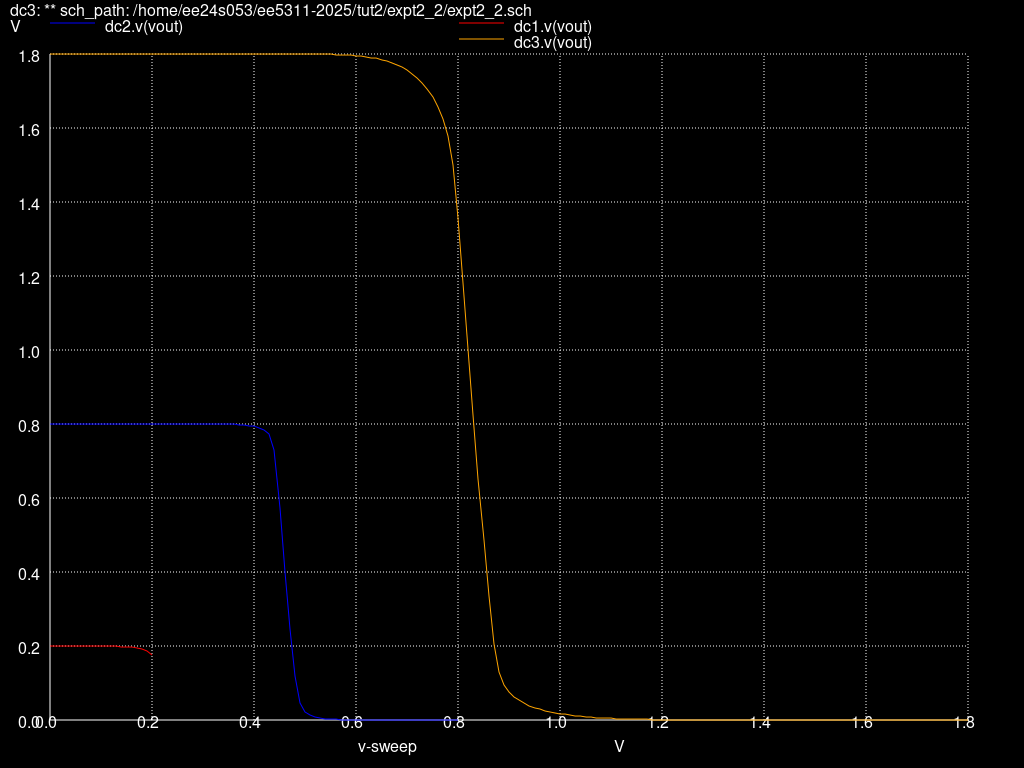
\includegraphics[width=0.49\linewidth]{tut2/reports/media/expt2_2_vtc.png} \\
Fig 8a: Output Voltages for a range of Supply Voltages & Fig 8b: Output Voltages for Selected Supply Voltages
\end{tabular}
\end{center}

\noindent We note that the inverter \emph{can not} can be used as an inverter for all these supply voltages, since the inverter threshold is not close to $V_{DD}/2$ for all these supply voltage levels. As the supply voltage decreases, we note that the $V_M$ increases, indicating that the pMOS needs to be up-sized.
\newline \newline

\noindent We analyze the DC characteristics of the same inverter for three different voltage levels - $0.2V$, $0.8V$ and $1.8V$. We obtain the plots in (fig. 8b) for the voltage transfer characteristics and the following plots for drain currents when operating at the said three voltage levels:


\begin{center}
\begin{tabular}{cc}
     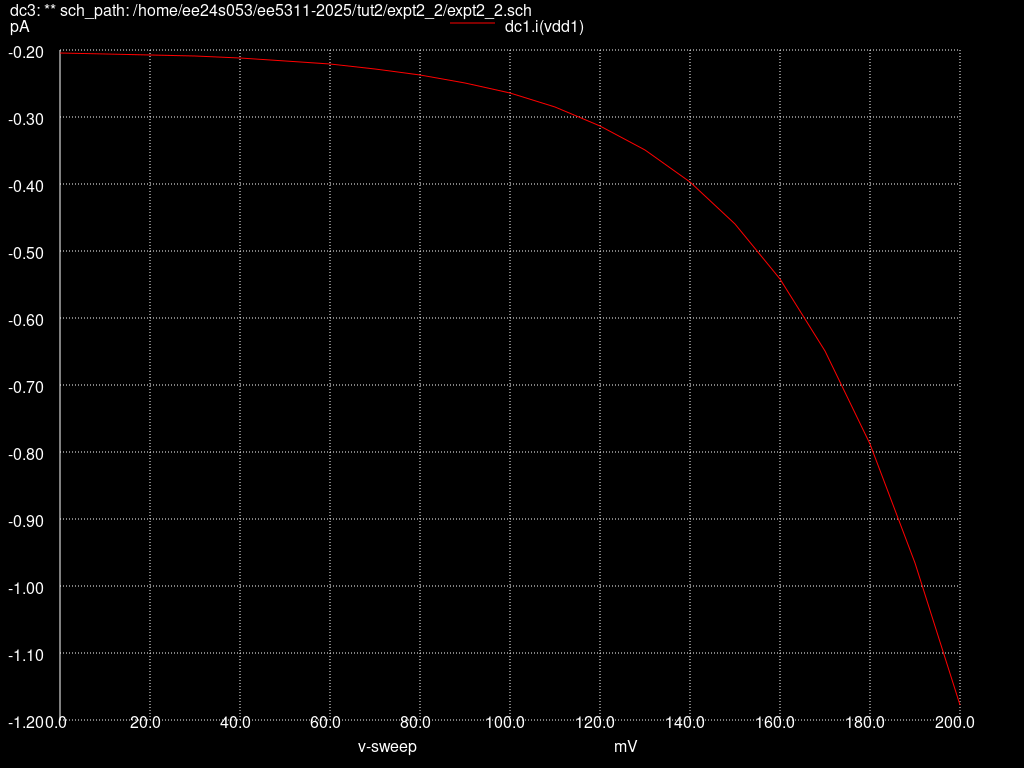
\includegraphics[width=0.49\linewidth]{tut2/reports/media/expt2_2_ids_0_2.png} &
     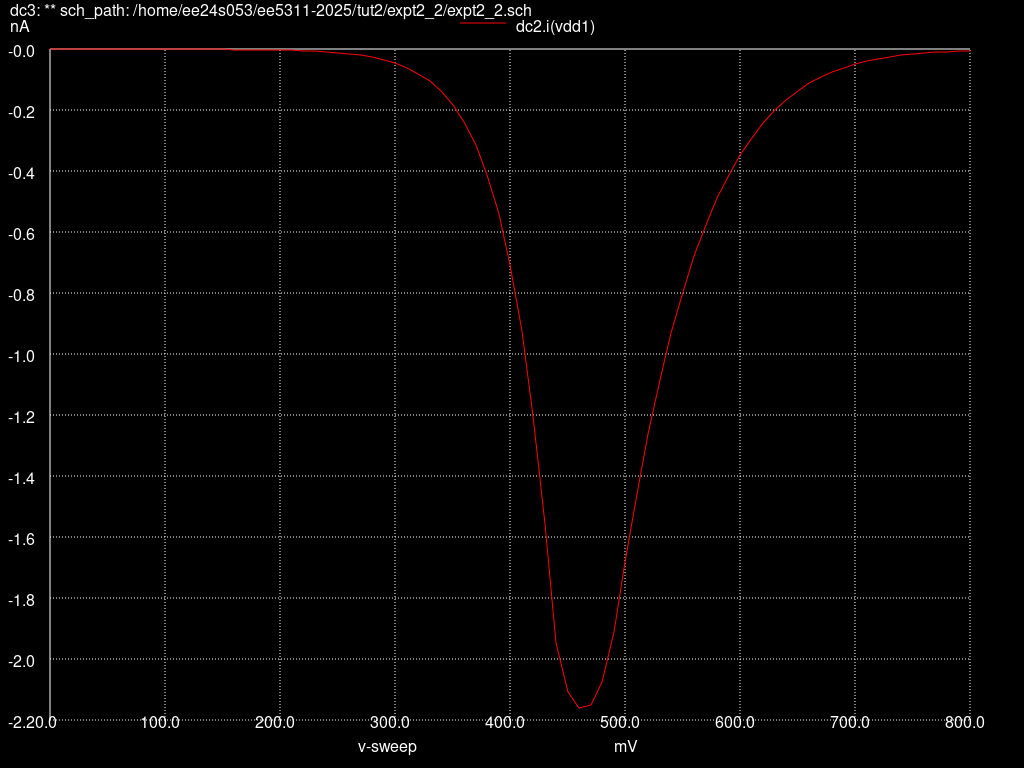
\includegraphics[width=0.49\linewidth]{tut2/reports/media/expt2_2_ids_0_8.png} \\
     Fig 9a: Drain Current against $V_{in}$ for $V_{DD} = 0.2V$ & Fig 9b: Drain Current against $V_{in}$ for $V_{DD} = 0.8V$
\end{tabular}
\\
\begin{tabular}{cc}
     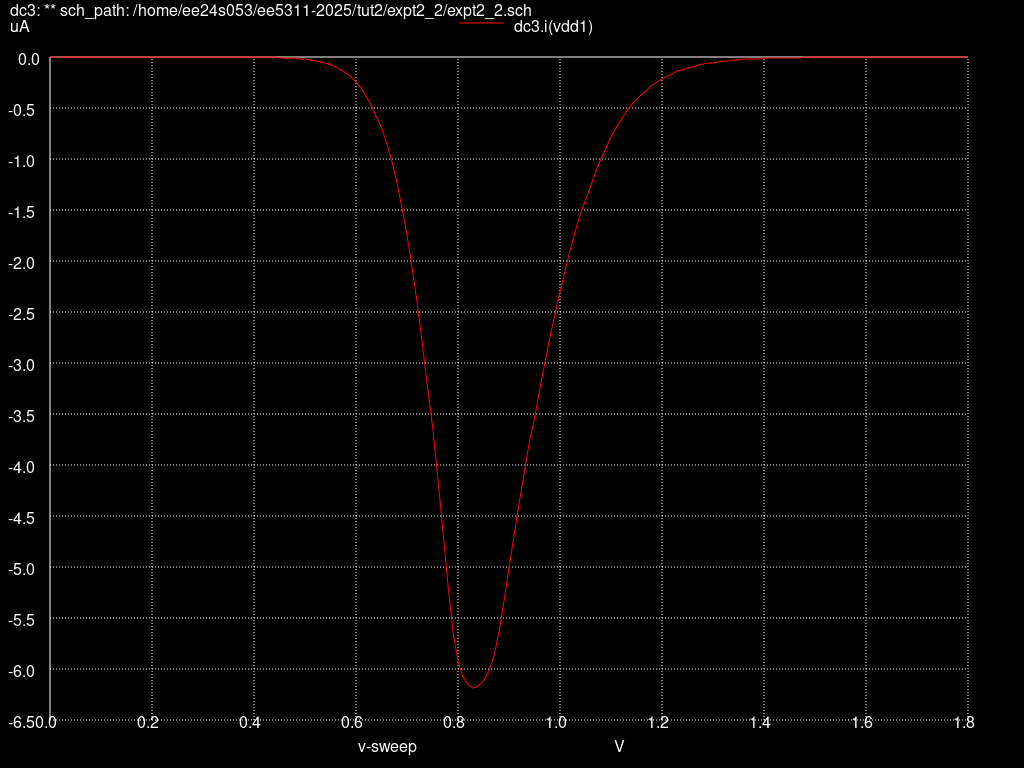
\includegraphics[width=0.49\linewidth]{tut2/reports/media/expt2_2_ids_1_8.png} &
     \\ Fig 9c: Drain Current against $V_{in}$ for $V_{DD} = 1.8V$
\end{tabular}
\end{center}

\noindent We make the following observations.

\begin{enumerate}
    \item The magnitude of drain current reduces drastically as the supply voltage is reduced.
    \item The inverter is still able to operate as an inverter as long as the supply voltage is larger than the transistor threshold voltage.
    \item The pMOS cannot pull the output voltage up for supply voltages below the transistor's threshold voltage. In order for the pMOS to be able to do that, we would need to model the circuit such that the pMOS is in the sub-threshold region when the nMOS is off/linear/saturated and matches the drain currents.
\end{enumerate}

\noindent The peak value of drain current in each of the three scenarios is:

\begin{enumerate}
    \item $I_{D,max} = -1.2 pA$ at $V_{DD} = 0.2 V$
    \item $I_{D,max} = -2.2 nA$ at $V_{DD} = 0.8 V$
    \item $I_{D,max} \approx -6.3 \mu A$ at $V_{DD} = 1.8 V$
\end{enumerate}

\noindent, The very first observation we make is that the $I_{D,max}$ is 3 orders of magnitude apart for the three given supply voltage levels. Upon comparing these values with (\ref{eq:expt2-idmax-subvt}), (\ref{eq:expt2-idmax-nearvt}), (\ref{eq:expt2-idmax-supervt}) we note that the values are comparable.

\end{document}
